\documentclass[a4paper,12pt,numbers=noenddot]{scrreprt}

\usepackage{lipsum}
\usepackage{graphicx}
\usepackage[left=2cm, right=2cm, bottom=3cm, top=3cm]{geometry}
\usepackage[onehalfspacing]{setspace}
\usepackage[utf8]{inputenc}
\usepackage{float}
\usepackage{enumerate}
\usepackage{url}
\usepackage{hyperref}
\usepackage[nohyperlinks]{acronym}
\usepackage{graphicx}
\usepackage[]{xcolor}
\usepackage{nameref}
\usepackage{footnote}
\usepackage{tikz}
\usepackage{pgfplots}
\usepackage{todonotes}
\usepackage{lipsum}
\usepackage[english]{babel}
\usepackage[backend=biber]{biblatex}
\addbibresource{Bibliography.bib}
\usepackage{amsmath}
\usepackage{wrapfig}
\usepackage{textgreek}
\usepackage{csquotes}
\usepackage{multirow}
\pgfplotsset{compat=1.18}
\usepackage{scrhack} 
\usepackage{tikz}
\setlength{\marginparwidth}{2cm}
\usepackage{scrlayer-scrpage}
\renewcommand*{\chapterpagestyle}{scrheadings}
\clearpairofpagestyles
\ohead{\normalfont Page~\pagemark}
\chead{\normalfont Assignment 2}
\ihead{\normalfont \rightmark}
\ofoot{\normalfont \leftmark}
\cfoot{\normalfont Fanò, Mecatti, Stano}
\ifoot{\normalfont \myauthor} 
\KOMAoptions{headsepline=true,footsepline=true}
\renewcommand*{\chapterheadstartvskip}{\vspace*{-.4cm}}
\renewcommand*{\chapterheadendvskip}{\vspace{.5cm}}
\setlength{\parindent}{0pt}
\setkomafont{chapter}{\LARGE}
\setkomafont{section}{\Large}
\setkomafont{subsection}{\large}
\setkomafont{subsubsection}{\normalsize}
\setkomafont{paragraph}{\normalsize}
\setkomafont{subparagraph}{\small}
\usetikzlibrary{shapes, arrows.meta, positioning}



\begin{document}

\chapter*{Introduction and Overview}

    \section*{Abstract}
    
        This assignment covers some common problems of compilers' middle-end, namely \textbf{Very Busy Expressions -- VBE}, \textbf{Dominator Analysis -- DA} and \textbf{Constant Propagation -- CP}, addressing them with DFA -- Data Flow Analysis -- framework.
    
    \section*{Summary}
    
        All the aforementioned problems can be framed as \textbf{data-flow problems}; solving them would allow us to drive new optimizations.

        The table's In/Out notation \ref{tab:summary_table} is chosen under the assumption that data flow direction doesn't affect blocks' input-output naming, i.e. the \textbf{input} of a block is always its \textbf{entry point} and the \textbf{output} of a block is always its \textbf{exit point}, regardless of the problem-specific \textit{direction}.

        \vspace{1cm}

        \begin{table}[H]
            \centering
            \resizebox{17.5cm}{!}{
            \begin{tabular}{|c|c|c|c|}
                \hline
                \textbf{} & \textbf{Very Busy Expressions} & \textbf{Dominators Analysis} & \textbf{Constant Propagation} \\
                \hline
                \textbf{Domain} & Set of expressions & Set of basic blocks & Set of tuples (var, lit) \\
                \textbf{Direction} & Backward & Forward & Forward \\
                \textbf{Boundary Conditions} & $In[BB_{Exit}] = \emptyset$ & $Out[BB_{Entry}] = \{BB_{Entry}\}$ & $Out[BB_{Entry}] = \emptyset$ \\
                \textbf{Transfer Function} & $In[BB_i] = Gen[BB_i] \cup (Out[BB_i] \setminus Kill[BB_i])$ & $Out[BB_i] = In[BB_i] \cup \{BB_i\}$ & $Out[BB_i] = Gen[BB_i] \cup (In[BB_i] \setminus Kill[BB_i])$ \\
                \textbf{Meet Operator} & $\cap$ & $\cap$ & $\cap$ \\
                \textbf{Internal Points Init} & $In[BB_i] = \mathbb{U} \space \forall i \neq BB_{Exit}$ & $Out[BB_i] = \mathbb{U} \space \forall i \neq BB_{Entry}$ & $Out[BB_i] = \mathbb{U} \forall i \neq BB_{Entry}$ \\
                \hline
            \end{tabular}
            }
            \caption{DFA Framework Summary Table}
            \label{tab:summary_table}
        \end{table}

\chapter*{Very Busy Expressions}

    \section*{Problem Definition}
    
        DEF. An expression is \textbf{very busy} in a given point \textit{p} \textbf{if and only if}, regardless of the path taken after \textit{p} -- i.e. for each path taken from \textit{p} to \textit{Exit} -- , the expression is used before any of its operands is \textbf{redefined} (since, as a result, the expression is invalid).

        Figuring out which expressions are \textbf{busy} in \textit{p}, would enable us to hoist the expression itself to the point \textit{p}.

    \section*{DFA Solution}
    
        We defined the problem's \textbf{domain} as a \textbf{static set of expressions}, which is made up of all RHS expressions in the \textbf{CFG}.
    
        The data flow direction is \textbf{backward}, since we only care about expressions that appear in the "future".
    
        Set intersection is the \textbf{meet operator} that better fit the definition: \textit{"[...] for each path from p to Exit [...]"}.
    
        Given that kind of meet operator, along with the need to keep the intersection with uncomputed interior points neutral, we opted for an initialization according to the following formula: $In[BB_i] = \mathbb{U} \space \forall i \neq Exit$.
    
        The analysis is kick-started by $In[BB_{Exit}] = \emptyset$, and equivalently $Out[BB_{Exit}] = \emptyset$.

    \subsection*{Transfer Function's Sets Definition}
    
        Each basic block $BB_i$ \textbf{inherits} a set of expressions from its \textbf{successor} $BB_{i+1}$; this set makes up the output set (input from expressions-propagation POV) of block $B_i$: $$Out[BB_i] = In[BB_{i+1}] \; \forall BB_i \in CFG : i \neq Exit$$
        
        Also, each block \textbf{kills} the set of expressions invalidated by its internal definitions. An expression $E = OP1 \oplus OP2$ is killed by a basic block BB if either \textbf{OP1 or OP are defined inside the block}: 
        $$Kill[BB_i] = \{ E = OP1 \oplus OP2 : OP1 \; redefined \wedge OP2 \; redefined \} \; \forall BB_i \in CFG$$

        Lastly, the \textbf{Gen-set} is defined as the set of expressions that appear as right-hand-side of BB's internal definitions: 
        $$Gen[BB_i] = \{ OP1_j \oplus OP2_j : E_j = OP1_j \oplus OP2_j \forall E_j \in BB_i\} \; \forall BB_i \in CFG$$

    \section*{Illustrative Iteration}

        \vspace{1cm}
    
        \begin{figure}[H]
            \centering
            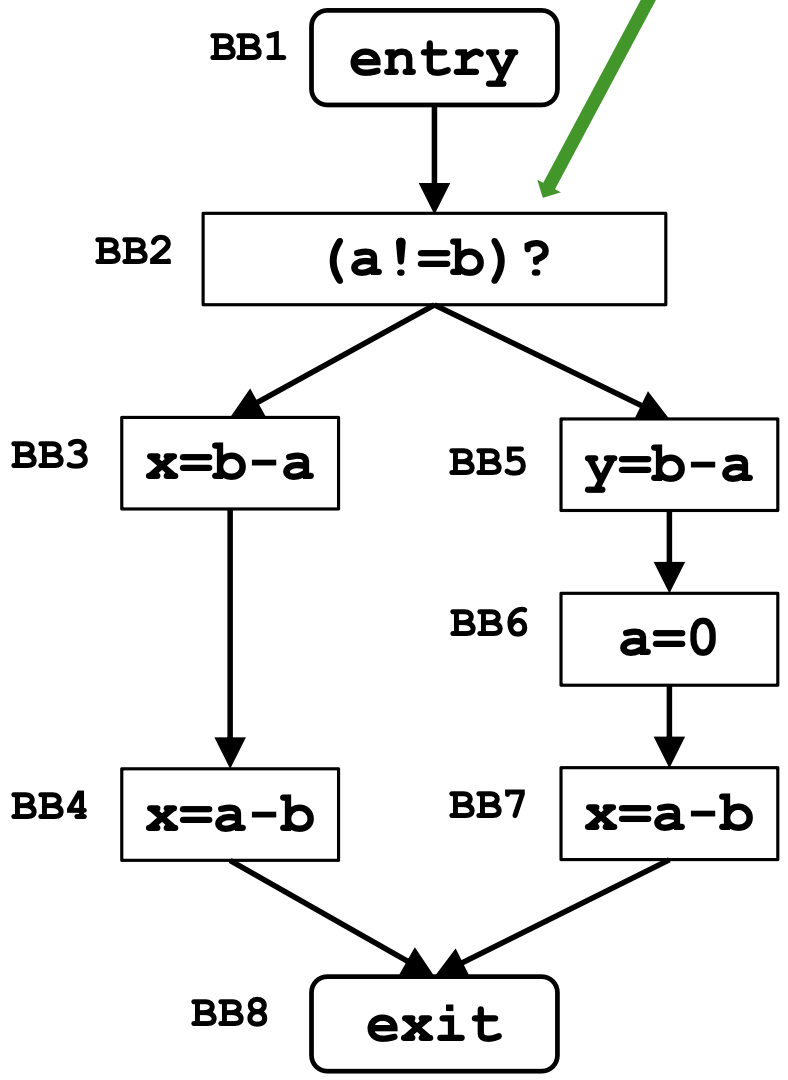
\includegraphics[width=0.3\linewidth]{assets/vbe.png}
            \caption{Reference CFG}
            \label{fig:vbe_iteration_image}
        \end{figure}

        \vspace{1cm}

        \begin{table}[H]
            \centering
            \begin{tabular}{|c|c|c|}
                \hline
                \textbf{Basic Block Name} & \textbf{Gen(BB)} & \textbf{Kill(BB)} \\
                \hline
                \textbf{Entry} & Ø & Ø \\
                \textbf{BB2} & Ø & Ø \\
                \textbf{BB3} & b - a & Ø \\
                \textbf{BB4} & a - b & Ø \\
                \textbf{BB5} & b - a & Ø \\
                \textbf{BB6} & Ø & b - a , a - b\\
                \textbf{BB7} & a - b & Ø \\
                \textbf{Exit}  & Ø & Ø \\
                \hline
            \end{tabular}
            \caption{Gen-Kill Table}
            \label{tab:vbe_gen_kill_table}
        \end{table}

        \vspace{1cm}

        \begin{table}[H]
            \centering
            \begin{tabular}{|c|c|c|}
                \hline
                \textbf{Node} & \textbf{In(BB)} & \textbf{Out(BB)} \\
                \hline
                \textbf{Entry} & b - a & b - a \\
                \textbf{BB2}   & b - a & b - a \\
                \textbf{BB3}   & b - a , a - b  & a - b \\
                \textbf{BB4}   & a - b & Ø \\
                \textbf{BB5}   & b - a & Ø \\
                \textbf{BB6}   & Ø & a - b\\
                \textbf{BB7}   & a - b & Ø \\
                \textbf{Exit}  & Ø & Ø \\
                \hline
            \end{tabular}
            \caption{Input-Output Table for Iteration 1}
            \label{tab:vbe_input_output_table}
        \end{table}

        The execution stops after the first iteration since there are no back-edges in the CFG.

\chapter*{Dominator Analysis}

    \section*{Problem Definition}

        In a \textbf{CFG}, we say that a node \textit{X} \textbf{dominates} another node \textit{Y} if node \textit{X} appears in every path of the graph that leads from the \textbf{Entry} block to block \textit{Y}.
        \begin{itemize}
            \item We annotate each basic block $B_i$ with a set \textbf{DOM[$B_i$]}
            \begin{itemize}
                \item $B_i \in DOM[B_j]$, if and only if $B_i$ dominates $B_j$.
            \end{itemize}
            \item By definition, a \textbf{node dominates itself}
                \begin{itemize}
                    \item $B_i \in DOM[B_i]$
                \end{itemize}
        \end{itemize}

    \section*{DFA Solution}
    
        We defined the domain of the problem as a \textbf{static set of blocks}, which are the \textbf{nodes} of the \textbf{CFG}.
        
        The data flow direction is \textbf{forward}, since the concept of dominance is defined in the "past".
        
        The \textbf{meet operator} can be inferred by the definition: \textit{[...] for each path from Entry to Y [...]}, is equivalent to set intersection.
        
        Given that kind of meet operator, along with the need to keep the \textbf{intersection} with uncomputed interior points \textbf{neutral}, interior points are initialized according to the following formula: 
        $Out[BB_i] = \mathbb{U} \space \; \forall i \neq Entry$.
        
        The analysis is kick-started by $Out[BB_{Entry}] = Entry$, since according to the definition: \textit{[...] each node dominates itself [...]}.

        \subsection*{Transfer Function's Sets Definition}
        
            Each basic block $BB_i$ \textbf{inherits} a set of expressions from its \textbf{predecessor} $BB_{i-1}$; this set makes up the block's input set $B_i$: $$In[BB_i] = Out[BB_{i-1}] \; \forall BB_i \in CFG : i \neq Entry$$
        
            The \textbf{kill set is empty} because, considering each node $BB_i$, name conflicts don't show up. Each node \textbf{adds} \textbf{itself} to the dominators' set without deleting other elements. As a consequence, the only reason to remove an element from the dominators' set is due to the \textbf{intersection} between the \textbf{dominators' sets coming from different paths}.  $$Kill[BB_i] = \emptyset \; \forall BB_i \in CFG$$

            Lastly, as mentioned above, the \textbf{Gen-set} of the $BB_i$ is defined as a set with only the $BB_i$ since \textbf{each node dominates itself}: $$Gen[BB_i] = \{ BB_i \} \; \forall BB_i \in CFG$$ 

    \section*{Illustrative Iteration}

        \vspace{1cm}
        
        \begin{center}
            \begin{tikzpicture}[node distance=0.75cm and 0.5cm][H]
            
                % Nodes
                \node (A) [circle, draw, minimum size = 1.5cm] {A};
                \node (B) [below left=of A, circle, draw, minimum size = 1.5cm] {B};
                \node (C) [below right=of A, circle, draw, minimum size = 1.5cm] {C};
                \node (D) [below left=of C, circle, draw, minimum size = 1.5cm] {D};
                \node (E) [below right=of C, circle, draw, minimum size = 1.5cm] {E};
                \node (F) [below right=of D, circle, draw, minimum size = 1.5cm] {F};
                \node (G) [below=of F, circle, draw, minimum size = 1.5cm] {G};
    
                % Edges
                \draw[->] (A) -- (B);
                \draw[->] (A) -- (C);
                \draw[->] (C) -- (D);
                \draw[->] (C) -- (E);
                \draw[->] (D) -- (F);
                \draw[->] (E) -- (F);
                \draw[->] (F) -- (G);
                \draw[->] (B) to[out=270,in=150] (G);
            \end{tikzpicture}
        \end{center}

     \vspace{1cm}
        
        \begin{table}[H]
            \centering
            \begin{tabular}{|c|c|c|}
                \hline
                \textbf{Node} & \textbf{In(BB)} & \textbf{Out(BB)} \\
                \hline
                \textbf{A}   & Ø & A \\
                \textbf{B}   & A & A , B \\
                \textbf{C}   & A  & A , C \\
                \textbf{D}   & A , C & A , C , D \\
                \textbf{E}   & A , C & A , C , E \\
                \textbf{F}   & A , C & A , C , F\\
                \textbf{G}   & A & A , G \\
                \hline
            \end{tabular}
            \caption{Input-Output Table for Iteration 1}
            \label{tab:da_input_output_table}
        \end{table}

        The execution stops after the first iteration since there are no back-edges in the CFG.
        
    \subsection*{Dominator Tree}

        Below is reported the \textbf{Dominator Tree} obtained by applying the algorithm of \textbf{Dominator Analysis}. The following graph is pretty self-explainatory, it represents the \textbf{dominance relationship} between \textbf{parent-child nodes}, and it follows the rules of the Iput/Output table, where each parent node dominates their childs and each node dominates itself.  
        
        \vspace{1cm}
        
        \begin{center}
            \begin{tikzpicture}[node distance=1.75cm and 1.25cm][H]
            
                % Nodes
                \node (A) [circle, draw, minimum size = 1.5cm] {\textbf{A}};
                \node (G) [below left=of A, circle, draw,  minimum size = 1.5cm] {\textbf{G}};
                \node (B) [below=of A, circle, draw,  minimum size = 1.5cm] {\textbf{B}};
                \node (C) [below right=of A, circle, draw, minimum size = 1.5cm] {\textbf{C}};
                \node (D) [below left=of C, circle, draw,  minimum size = 1.5cm] {\textbf{D}};
                \node (E) [below=of C, circle, draw,  minimum size = 1.5cm] {\textbf{E}};
                \node (F) [below right=of C, circle, draw,  minimum size = 1.5cm] {\textbf{F}};
    
                % Edges
                \draw[->] (A) -- (B);
                \draw[->] (A) -- (C);
                \draw[->] (A) -- (G);
                \draw[->] (C) -- (D);
                \draw[->] (C) -- (E);
                \draw[->] (C) -- (F);
            \end{tikzpicture}
        \end{center}

\chapter*{Constant Propagation}
\label{chap:Constant Propagation}
    \section*{Problem Definition}

        The goal of \textbf{constant propagation} is to determine in which points of the program variables have a constant value.
        
        The information to be computed for each node \textbf{n} of the Control Flow Graph (\textbf{CFG}) is a set of pairs in the form $<\textbf{variable,\; constant value}>$.
        
        If we have the pair $<\textbf{x,\; c}>$ at node \textit{n}, it means that x is guaranteed to have the value \textit{c} every time \textit{n} is reached during program execution.

    
    \section*{DFA Solution}

        This solution works under the \textbf{assumption that the transfer function can integrate some piece of logic}. In particular, some sort of expression-solving mechanism is needed to compute expressions such as $k+2$, expanding them to a constant value. For instance, $k+2$ expression in BB3 of Figure \ref{fig:cp_iteration_image}, should become $4$ after passing through BB3's transfer function.

        Consequently, the domain of this problem, defined as the set of tuples $<\textbf{variable, constant value}>$, is \textbf{variable-sized}, thus making unfeasible a bit-vector implementation. This is due to the fact we have \textbf{no prior knowledge} about the number of tuples that could appear while algorithm is executing.
        As a matter of fact, by solving an expression, a new tuple could be generated at "runtime".

        For a solution that admits a \textbf{bit-vector implementation}, have a look at our considerations in the next \textbf{\autoref{chap:Constant Propagation with Fixed-size Domain}}.
        
        We defined the \textbf{domain} of the problem as a \textbf{set of definitions with literal or constant values as RHS, represented as tuples} $<\textbf{variable, \;constant \;value}>$.
        
        The data flow is oriented \textbf{forward} because it's essential to reference past values of variables to ensure which ones remain constant.
        
        The \textbf{meet operator} is equivalent to \textbf{set intersection} because a variable is deemed constant only if it's confirmed across every potential path.
        
        Given that kind of meet operator, along with the need to keep the intersection with uncomputed interior points neutral, \textbf{interior points} are initialized according to the following formula: $Out[BB_i] = \mathbb{U} \; \forall i \neq Entry$.
        
        The analysis is kick-started by $Out[BB_{Entry}] = \emptyset$.
        
        The solution uses a \textbf{dynamic sized dictionary} to keep track of the variable's value which was computed using operands with constant values. Each dictionary element's key consists of a pair $<\textbf{variable,\; constant \; value}>$ associated to a boolean value representing whether the variable assumes the constant value at a specific point of the program.
        
    \subsection*{Transfer Function's Sets Definition}

        The \textbf{Kill} and \textbf{Gen-set} is defined using \textbf{tuples} $<\textbf{variable,\; expression}>$ to differentiate definitions of the same variables which could have the same result during the execution of the program. The Transfer Function will compute the result of the expression and insert in the dictionary the tuple $<\textbf{variable,\; constant \; value}>$ obtained. If at a certain point \textit{p} of the program the input dictionary does not contain some of the variables in the expression that needs to be computed, the tuple $<variable,\; expression>$ is discarded from the output set. 
        
        Each basic block $BB_i$ inherits a set of expressions from its \textbf{predecessor} $BB_{i-1}$; this set makes up the block's input set $B_i$: $$In[BB_i] = Out[BB_{i-1}] \; \forall BB_i \in CFG : i \neq Entry$$
        
        Also, each block \textbf{kills (globally)} the tuples $<\textbf{variable,\; expression}>$ invalidated by its internal definitions. A tuple $<\textbf{variable,\; expression}>$ is killed by a basic block \textbf{BB} if the variable is \textbf{defined} inside the block: $$Kill[BB_i] = \{ <variable,\; expression> : \; variable \; redefined \} \; \forall BB_i \in CFG$$

        In other words, a tuple is killed if it is shadowed by a new definition of the variable, which would make the previous definition (the definition that generate) invalid.

        Lastly, the \textbf{Gen-set} is defined as the set of tuple $<\textbf{variable,\; expression}>$ whenever the BB's internal definition of the variable is a \textit{constant expression}, or rather a \textbf{binary expression} where both operands are \textbf{variables} whose constant value is \textbf{known} or a \textbf{literal}.

        Let's define \textit{K} as a set of constant values, and \textit{k} as a constant value, $\forall k \in K$, we can declare an \textit{Operand} with constant value $k$ as \textit{$Op_k$}.
        
        The \textbf{Gen-set} based on these assumptions is the following: $$Gen[BB_i] = \{ <variable,\; expression > : \; \forall E_j = OP_{k_\alpha} \; \oplus \; OP_{k_\beta} \; \in BB_i\; \wedge \; Op_k \; \forall k \in K \}$$
        $$\forall BB_i \; \in \; CFG, \; \forall \alpha, \; \beta \; \in \; \mathbb{N}, \; \forall k \in K$$

        To cope with cases of redefinition of a previous definition's RHS -- e.g. $a=1$ after Figure \ref{fig:cp_iteration_image}'s BB7 --, the concept of \textit{definition freshness} is introduced. In order to avoid \textbf{conflicts}, Transfer Function's \textbf{union operator} must take into consideration that tuples coming from the gen-set are the newer ones, so they are more \textit{fresh} than the tuples coming from the $(In[BB_I] \setminus Kill[BB_i])$ set, favouring the former over the latter. The priority is given to gen-set's tuples by discarding tuples which have the same variable as first element, but are no longer fresh -- i.e. in case of a conflict, only the fresher tuple should survive.
        
    \section*{Illustrative Iteration}

        \begin{figure}[H]
            \centering
            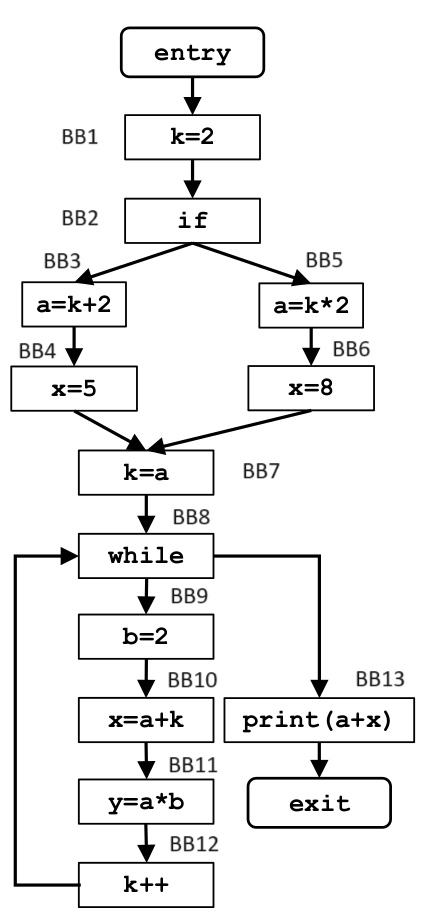
\includegraphics[width=0.4\linewidth]{assets/cp.png}
            \caption{Reference CFG}
            \label{fig:cp_iteration_image}
        \end{figure}
        
        \begin{table}[H]
            \centering
            \resizebox{8.5cm}{!}{
            \begin{tabular}{|c|c|c|}
                \hline
                \textbf{Basic Block Name} & \textbf{Gen(BB)} & \textbf{Kill(BB)} \\
                \hline
                \textbf{BB1}  & $<k, 2>$ & $<k, a> , <k, k++>$ \\
                \textbf{BB2}  & Ø & Ø \\
                \textbf{BB3}  & $<a, k+2>$ & $<a, k*2>$ \\
                \textbf{BB4}  & $<x, 5>$ & $<x, 8>$ , $<x, a+k>$ \\
                \textbf{BB5}  & $<a , k*2>$ & $<a, k+2>$ \\
                \textbf{BB6}  & $<x, 8>$ & $<x, 5>$ , $<x, a+k>$ \\
                \textbf{BB7}  & $<k, a>$ & $<k, 2>$ , $<k, k++>$ \\
                \textbf{BB8}  & Ø & Ø \\
                \textbf{BB9}  & $<b, 2>$ & Ø \\
                \textbf{BB10} & $<x, a+k>$ & $<x, 5>$ , $<x , 8>$ \\
                \textbf{BB11} & $<y, a*b>$ & Ø \\
                \textbf{BB12} & $<k, k++>$ & $<k, 2>$ , $<k, a>$ \\
                \textbf{BB13} & Ø & Ø \\
                \hline
            \end{tabular}
            }
            \caption{Gen-Kill Table}
            \label{tab:cp_gen_kill_table}
        \end{table}

    \subsection*{Iteration 1}
    
        \vspace{0.1cm}
        
        \begin{table}[H]
            \centering
            \resizebox{0.8\textwidth}{!}{
            \begin{tabular}{|c|c|c|}
                \hline
                \textbf{Node} & \textbf{In(BB)} & \textbf{Out(BB)} \\
                \hline
                \textbf{Entry} & Ø & Ø \\
                \textbf{BB1}   & Ø & $<k, 2>$ \\
                \textbf{BB2}   & $<k, 2>$ & $<k, 2>$ \\
                \textbf{BB3}   & $<k, 2>$ & $<a, 4>$ , $<k, 2>$  \\
                \textbf{BB4}   & $<a, 4>$ , $<k, 2>$ & $<a, 4>$ , $<k, 2>$ , $<x, 5>$ \\
                \textbf{BB5}   & $<k, 2>$ &  $<a, 4>$ , $<k, 2>$ \\
                \textbf{BB6}   & $<a, 4>$ , $<k, 2>$ & $<a, 4>$ , $<k, 2>$ , $<x, 8>$ \\
                \textbf{BB7}   & $<a, 4>$ , $<k, 2>$ & $<a, 4>$ , $<k, 4>$ \\
                \textbf{BB8}   & $<a, 4>$ , $<k, 4>$ & $<a, 4>$ , $<k, 4>$ \\
                \textbf{BB9}   & $<a, 4>$ , $<k, 4>$ & $<a, 4>$ , $<b, 2>$ , $<k, 4>$ \\
                \textbf{BB10}  & $<a, 4>$ , $<b, 2>$ , $<k, 4>$ & $<a, 4>$ , $<b, 2>$ , $<k, 4>$ , $<x, 8>$ \\
                \textbf{BB11}  & $<a, 4>$ , $<b, 2>$ , $<k, 4>$ , $<x, 8>$ & $<a, 4>$ , $<b, 2>$ , $<k, 4>$ , $<x, 8>$ , $<y, 8>$ \\
                \textbf{BB12}  & $<a, 4>$ , $<b, 2>$ , $<k, 4>$ , $<x, 8>$ , $<y, 8>$ & $<a, 4>$ , $<b, 2>$ , $<k, 5>$ , $<x, 8>$ , $<y, 8>$ \\
                \textbf{BB13}  & $<a, 4>$ , $<k, 4>$ & $<a, 4>$ , $<k, 4>$ \\
                \textbf{Exit}  & $<a, 4>$ , $<k, 4>$ & \\
                \hline
            \end{tabular}
            }
            \caption{Input-Output Table, Iteration 1}
            \label{tab:cp_input_output_table1}
        \end{table}

        The execution continues after the first iteration since there are back-edges in the CFG.
    
    \subsection*{Iteration 2}

        \vspace{0.1cm}

        \begin{table}[H]
            \centering
            \resizebox{8.5cm}{!}{
            \begin{tabular}{|c|c|c|}
                \hline
                \textbf{Node} & \textbf{In(BB)} & \textbf{Out(BB)} \\
                \hline
                \textbf{Entry} & Ø & Ø \\
                \textbf{BB1}   & Ø & $<k, 2>$ \\
                \textbf{BB2}   & $<k, 2>$ & $<k, 2>$ \\
                \textbf{BB3}   & $<k, 2>$ & $<a, 4>$ , $<k, 2>$  \\
                \textbf{BB4}   & $<a, 4>$ , $<k, 2>$ & $<a, 4>$ , $<k, 2>$ , $<x, 5>$ \\
                \textbf{BB5}   & $<k, 2>$ &  $<a, 4>$ , $<k, 2>$ \\
                \textbf{BB6}   & $<a, 4>$ , $<k, 2>$ & $<a, 4>$ , $<k, 2>$ , $<x, 8>$ \\
                \textbf{BB7}   & $<a, 4>$ , $<k, 2>$ & $<a, 4>$ , $<k, 4>$ \\
                \textbf{BB8}   & $<a, 4>$ & $<a, 4>$ \\
                \textbf{BB9}   & $<a, 4>$ & $<a, 4>$ , $<b, 2>$ \\
                \textbf{BB10}  & $<a, 4>$ , $<b, 2>$ & $<a, 4>$ , $<b, 2>$ \\
                \textbf{BB11}  & $<a, 4>$ , $<b, 2>$ & $<a, 4>$ , $<b, 2>$ , $<y, 8>$ \\
                \textbf{BB12}  & $<a, 4>$ , $<b, 2>$ , $<y, 8>$ & $<a, 4>$ , $<b, 2>$ , $<y, 8>$ \\
                \textbf{BB13}  & $<a, 4>$ & $<a, 4>$ \\
                \textbf{Exit}  & $<a, 4>$ & \\
                \hline
            \end{tabular}
            }
            \caption{Input-Output Table, Iteration 2}
            \label{tab:cp_input_output_table2}
        \end{table}
            
            The tuple of the gen set $<\textbf{k,\; k++}>$ is removed from the input set of BB8 by the intersection between the output sets of BB7 and BB12. The final solution contains only the variables whose value is always constant in a specific point of the program, the variable \textit{k} has a value which changes from one iteration to another thus it has to be removed.
            In the BB10 the tuple of the gen set $<\textbf{x,\; a+k}>$ is discarded because the variable \textit{k} is not defined in the input dictionary.
    
    \subsection*{Iteration 3}

        \vspace{0.1cm}
        
        \begin{table}[H]
            \centering
            \resizebox{8.5cm}{!}{
            \begin{tabular}{|c|c|c|}
                \hline
                \textbf{Node} & \textbf{In(BB)} & \textbf{Out(BB)} \\
                \hline
                \textbf{Entry} & Ø & Ø \\
                \textbf{BB1}   & Ø & $<k, 2>$ \\
                \textbf{BB2}   & $<k, 2>$ & $<k, 2>$ \\
                \textbf{BB3}   & $<k, 2>$ & $<a, 4>$ , $<k, 2>$  \\
                \textbf{BB4}   & $<a, 4>$ , $<k, 2>$ & $<a, 4>$ , $<k, 2>$ , $<x, 5>$ \\
                \textbf{BB5}   & $<k, 2>$ &  $<a, 4>$ ; $<k, 2>$ \\
                \textbf{BB6}   & $<a, 4>$ , $<k, 2>$ & $<a, 4>$ , $<k, 2>$ , $<x, 8>$ \\
                \textbf{BB7}   & $<a, 4>$ , $<k, 2>$ & $<a, 4>$ , $<k, 4>$ \\
                \textbf{BB8}   & $<a, 4>$ & $<a, 4>$ \\
                \textbf{BB9}   & $<a, 4>$ & $<a, 4>$ , $<b, 2>$ \\
                \textbf{BB10}  & $<a, 4>$ , $<b, 2>$ & $<a, 4>$ , $<b, 2>$ \\
                \textbf{BB11}  & $<a, 4>$ , $<b, 2>$ & $<a, 4>$ , $<b, 2>$ , $<y, 8>$ \\
                \textbf{BB12}  & $<a, 4>$ , $<b, 2>$ , $<y, 8>$ & $<a, 4>$ , $<b, 2>$ , $<y, 8>$ \\
                \textbf{BB13}  & $<a, 4>$ & $<a, 4>$ \\
                \textbf{Exit}  & $<a, 4>$ & \\
                \hline
            \end{tabular}
            }
            \caption{Input-Output Table, Iteration 3}
            \label{tab:cp_input_output_table3}
        \end{table}

        The execution stops after the third iteration since there are no changes in the input and output sets.
    
        \newpage
        \chapter*{Constant Propagation With Fixed-size Domain}
        \label{chap:Constant Propagation with Fixed-size Domain}

        \section*{Problem Definition}

        The goal of \textbf{constant propagation} is to determine in which points of the program, a given variable, has a constant value.
        
        The information to be computed for each node \textbf{n} of the Control Flow Graph (\textbf{CFG}) is a set of pairs in the form $<\textbf{variable,\; literal}>$.
        
        If we have the pair $<\textbf{x,\; c}>$ at node \textit{n}, it means that x is guaranteed to have the value \textit{c} every time \textit{n} is reached during program execution.

        The main difference, compared to the problem of the previous \textbf{\autoref{chap:Constant Propagation}}, is that the domain set is composed by variables defined using only \textbf{literals} as RHS, therefore \textbf{expressions} are \textbf{excluded}.
        
        \section*{DFA Solution}
        
        We defined the \textbf{domain} of the problem as a \textbf{set of definitions with literal as RHS, represented as tuples} $<\textbf{variable, \; literal}>$.
        
        The data flow is oriented \textbf{forward} because it's essential to reference past values of variables to ensure which ones remain constant.
        
        The \textbf{meet operator} is equivalent to \textbf{set intersection} because a variable is deemed constant only if it's confirmed across every potential path.
        
        Given that kind of meet operator, along with the need to keep the intersection with uncomputed interior points neutral, \textbf{interior points} are initialized according to the following formula: $Out[BB_i] = \mathbb{U} \; \forall i \neq Entry$.
        
        The analysis is kick-started by $Out[BB_{Entry}] = \emptyset$.
        
    \subsection*{Transfer Function's Sets Definition}

        Each basic block $BB_i$ inherits a set of expressions from its \textbf{predecessor} $BB_{i-1}$; this set makes up the block's input set $B_i$: $$In[BB_i] = Out[BB_{i-1}] \; \forall BB_i \in CFG : i \neq Entry$$
        
        Also, each block \textbf{kills (globally)} the tuples $<\textbf{variable,\; literal}>$ invalidated by its internal definitions. A tuple $<\textbf{variable,\; literal}>$ is killed by a basic block \textbf{BB} if the variable is \textbf{redefined} inside the block: $$Kill[BB_i] = \{ <variable,\; literal> : \; variable \; redefined \; in\; BB_i\} \; \forall BB_i \in CFG$$

        In other words, a tuple is killed if it is shadowed by a new definition of the variable, which would make the previous definition (the definition that generate) invalid.

        Lastly, the \textbf{Gen-set} is defined as the set of tuple $<\textbf{variable,\; constant \; value }>$ whenever the BB's internal definition of the variable has a literal as RHS:
        $$Gen[BB_i] = \{ <variable,\; literal > : \; \forall \;variable := literal\; \in BB_i\;\} \; \forall BB_i \in CFG$$
        
    \section*{Illustrative Iteration}

        \begin{figure}[H]
            \centering
            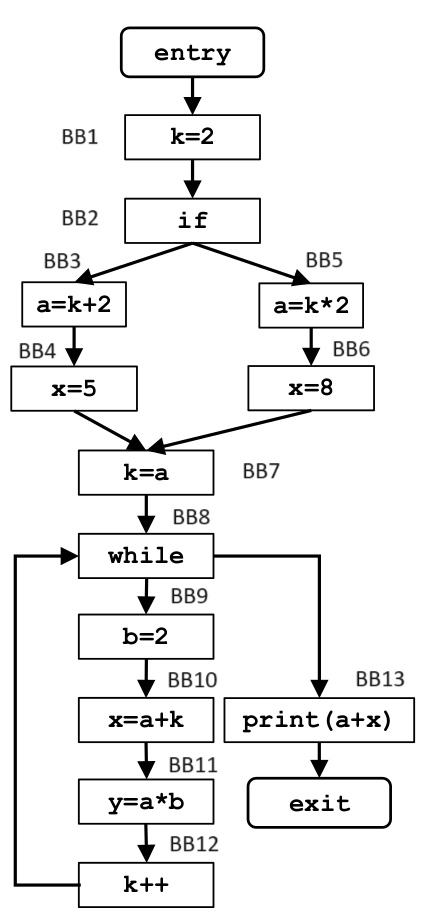
\includegraphics[width=0.3\linewidth]{assets/cp.png}
            \caption{Reference CFG}
            \label{fig:cp_iteration_image}
        \end{figure}
        
        \vspace{1cm}

        \begin{table}[H]
            \centering
            \resizebox{8.5cm}{!}{
            \begin{tabular}{|c|c|c|}
                \hline
                \textbf{Basic Block Name} & \textbf{Gen(BB)} & \textbf{Kill(BB)} \\
                \hline
                \textbf{BB1}  & $<k, 2>$ & Ø \\
                \textbf{BB2}  & Ø & Ø \\
                \textbf{BB3}  & Ø & Ø \\
                \textbf{BB4}  & $<x, 5>$ & $<x, 8>$ \\
                \textbf{BB5}  & Ø & Ø \\
                \textbf{BB6}  & $<x, 8>$ & $<x, 5>$ \\
                \textbf{BB7}  & Ø & $<k, 2>$ \\
                \textbf{BB8}  & Ø & Ø \\
                \textbf{BB9}  & $<b, 2>$ & Ø \\
                \textbf{BB10} & Ø & $<x, 5>$ , $<x , 8>$ \\
                \textbf{BB11} & Ø & Ø \\
                \textbf{BB12} & Ø & $<k, 2>$ \\
                \textbf{BB13} & Ø & Ø \\
                \hline
            \end{tabular}
            }
            \caption{Gen-Kill Table}
            \label{tab:cp_gen_kill_table}
        \end{table}


    \subsection*{Iteration 1}
    
        \vspace{1cm}

         \begin{table}[H]
            \centering
            \resizebox{8.5cm}{!}{
            \begin{tabular}{|c|c|c|}
                \hline
                \textbf{Basic Block Name} & \textbf{In(BB)} & \textbf{Out(BB)} \\
                \hline
                \textbf{Entry}  & Ø & Ø \\
                \textbf{BB1}    & Ø & $<k, 2>$ \\
                \textbf{BB2}    & $<k, 2>$ & $<k, 2>$ \\
                \textbf{BB3}    & $<k, 2>$ & $<k, 2>$ \\
                \textbf{BB4}    & $<k, 2>$ & $<k, 2>$ , $<x, 5>$ \\
                \textbf{BB5}    & $<k, 2>$ & $<k, 2>$ \\
                \textbf{BB6}    & $<k, 2>$ & $<k, 2>$ , $<x, 8>$ \\
                \textbf{BB7}    & $<k, 2>$ & Ø \\
                \textbf{BB8}    & Ø & Ø \\
                \textbf{BB9}    & Ø & $<b, 2>$\\
                \textbf{BB10}   & $<b, 2>$ & $<b, 2>$ \\
                \textbf{BB11}   & $<b, 2>$ & $<b, 2>$ \\
                \textbf{BB12}   & $<b, 2>$ & $<b, 2>$ \\
                \textbf{BB13}   & Ø & Ø \\
                \textbf{Exit}   & Ø &  \\
                \hline
            \end{tabular}
            }
            \caption{Input-Output Table, Iteration 1}
            \label{tab:cp_gen_kill_table}
        \end{table}

    \subsection*{Iteration 2}
    
        \vspace{1cm}

         \begin{table}[H]
            \centering
            \resizebox{8.5cm}{!}{
            \begin{tabular}{|c|c|c|}
                \hline
                \textbf{Basic Block Name} & \textbf{In(BB)} & \textbf{Out(BB)} \\
                \hline
                \textbf{Entry}  & Ø & Ø \\
                \textbf{BB1}    & Ø & $<k, 2>$ \\
                \textbf{BB2}    & $<k, 2>$ & $<k, 2>$ \\
                \textbf{BB3}    & $<k, 2>$ & $<k, 2>$ \\
                \textbf{BB4}    & $<k, 2>$ & $<k, 2>$ , $<x, 5>$ \\
                \textbf{BB5}    & $<k, 2>$ & $<k, 2>$ \\
                \textbf{BB6}    & $<k, 2>$ & $<k, 2>$ , $<x, 8>$ \\
                \textbf{BB7}    & $<k, 2>$ & Ø \\
                \textbf{BB8}    & Ø & Ø \\
                \textbf{BB9}    & Ø & $<b, 2>$\\
                \textbf{BB10}   & $<b, 2>$ & $<b, 2>$ \\
                \textbf{BB11}   & $<b, 2>$ & $<b, 2>$ \\
                \textbf{BB12}   & $<b, 2>$ & $<b, 2>$ \\
                \textbf{BB13}   & Ø & Ø \\
                \textbf{Exit}   & Ø &  \\
                \hline
            \end{tabular}
            }
            \caption{Input-Output Table, Iteration 2}
            \label{tab:cp_gen_kill_table}
        \end{table}

        The execution stops after the second iteration since there is only one back-edge and the intersection between $Out[BB_7]$ and $Out[BB_{12}]$, keeps $In[BB_8]$ empty.  
            
\end{document}
